\apendice{Documentación de usuario}

\section{Introducción}

\section{Requisitos de usuarios}

\section{Instalación}

\section{Manual del usuario}
\subsection{\textit{Alp’s Labeling Tool (ALT)}}

Para hacer el etiquetado, se va a hacer uso de \textit{Alp’s Labeling Tool (ALT)}.
Se trata de un etiquetador bastante sencillo, tanto de descargar como de usar.
\subsubsection{Software necesario}
Para poder etiquetar imágenes con esta herramienta vamos a necesitar 3 tipos de software:
\begin{itemize}
	\item Fiji \footnote{Descargar Fiji: http://fiji.sc/download}. Esta herramienta no precisa de instalación como tal, simplemente hay que descomprimir la carpeta que contiene la aplicación y ubicarla donde nos resulte más cómoda trabajar con ella.
	Para descargarla solo es necesario escoger el sistema operativo sobre el que vamos a trabajar.
	\item Action Bar \footnote{Descarga de Action Bar: https://goo.gl/dB6L1R}. Se trata de un plugin que hay que instalar directamente en la aplicación Fiji.
	\item ALT \footnote{Descarga de ALT: https://goo.gl/JgekhA}. Este macro plugin nos va ha permitir cargar las imágenes, dibujar etiquetas sobre ellas, poner nombres a dichas etiquetas, guardar la información, volver a cargarla y devolver las coordenadas en formato .txt o .csv.
\end{itemize}
Considerando que ya se tiene todo el software especificado,
la instalación de la aplicación se realizará siguiendo los siguientes pasos:
\begin{enumerate}
	\item Lo primero que se va a hacer es descomprimir la carpeta que contiene la aplicación de \textbf{Fiji} y ubicar dicha carpeta dónde nos sea más cómodo trabajar.
	\item A continuación, descomprimimos el plugin de \textbf{Action Bar} y lo dejamos dónde lo podamos usar.
	\item Vamos a iniciar la aplicación, la cual se encuentra dentro de la carpeta extraída. Veremos una barra de tareas como la mostrada en la imagen~\ref{fig:barra_de_tareas}
	\begin{figure}
		\centering
		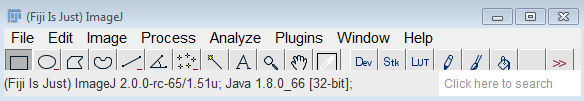
\includegraphics[width=0.7\linewidth]{img/barra}
		\caption{Barra de tareas de Fiji}
		\label{fig:barra_de_tareas}
	\end{figure}
	
	\item en la opción de menú "Plugins", vamos a seleccionar "Install Plugin..."	y tendremos que escoger el plugin "Action Bar" que habíamos descomprimido anteriormente. Tras esto reiniciamos la aplicación.
	\item Ahora abrimos la carpeta que contiene la aplicación que contiene la aplicación Fiji y abrimos el .zip que contiene ALT, la última descarga que hemos hecho. 
	\item Dentro del .zip de ALT hay una carpeta llamada "plugins". La seleccionamos y la arrastramos dentro de la carpeta de la aplicación.
	\item Reiniciar la aplicación en el caso de que estuviera abierta.
\end{enumerate}
Todo este proceso de instalación se puede ver en \href{https://www.youtube.com/watch?v=G6ib950iDvQ}{videotutoriales} que el propio desarrollador ha subido a Youtube.
\subsubsection{Uso de la aplicación}
\begin{itemize}
	\item \textbf{Uso de los plugins.} Una vez tenemos abierta la aplicación, nos dirigimos a la opción "Plugins" y en el desplegable y nos dirigimos al final de este. Seleccionamos "Alps Labeling Tool", como se muestra en la imagen \ref{fig:alpsltplugin}.
	Se nos abrirá una nueva barra de tareas como en la que se muestra en la imagen \ref{fig:alt}, con la que vamos a trabajar para hacer el etiquetado.
	\begin{figure}
		\centering
		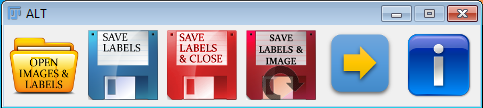
\includegraphics[width=0.7\linewidth]{img/alt}
		\caption{Barra de trabajo de ALT}
		\label{fig:alt}
	\end{figure}
	
	\begin{figure}
		\centering
		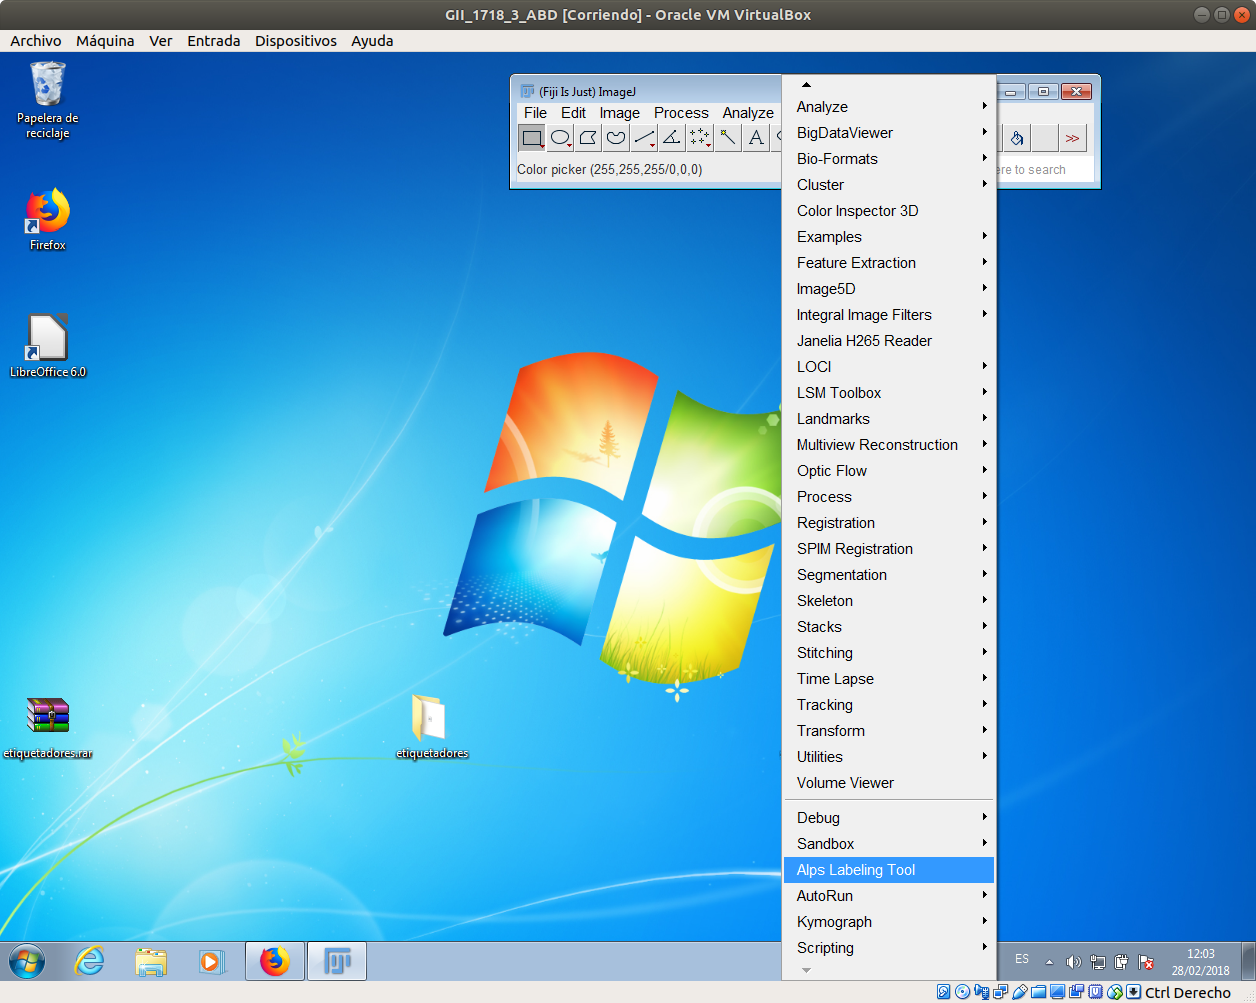
\includegraphics[width=0.7\linewidth]{img/AlpsLTPlugin}
		\caption{Plugin Alps Labeling Tool}
		\label{fig:alpsltplugin}
	\end{figure}
	Esta barra de trabajo contiene 6 funcionalidades básicas:
	\begin{enumerate}
		\item \textbf{OPEN IMAGES \& LABELS.} Con esta opción del menú vamos a seleccionar la imagen con la que vamos a trabajar. Lo ideal es seleccionar la primera imagen del directorio donde tengamos las imágenes para poder trabajar de forma ordenada, rápida y más segura.
		\item \textbf{SAVE LABELS.} Una vez hayamos realizado el etiquetado sobre la imagen podremos guardar en un .txt con las coordenadas de cada etiqueta de la imagen.
		\item \textbf{SAVE LABELS \& CLOSE.}Cuando ya hemos hecho el etiquetado sobre la imagen, si seleccionamos esta opción, nos permitirá guardar los datos de las etiquetas de la imagen y después cierra dicha imagen.
		\item \textbf{SAVE LABELS \& IMAGE.} Con esta opción podemos guardar la imagen con la información en otro directorio.
		\item \textbf{Flecha amarilla.} Nos carga la siguiente imagen del directorio.
		\item \textbf{Información.} Es la ayuda de la aplicación.
		
	\end{enumerate}
	
	\item \textbf{Cargar Imágenes.} Para poder trabajar etiquetando las imágenes, antes tenemos que cargarlas para visualizarlas. Para ello seleccionamos la opción \textit{OPEN IMAGES \& LABELS.}. Nos va a permitir navegar entre directorios para seleccionar finalmente qué imagen queremos etiquetar.
	Una vez esté la imagen abierta, la vista será similar a la mostrada en la imagen \ref{fig:etiquetado0}.
	\begin{figure}
		\centering
		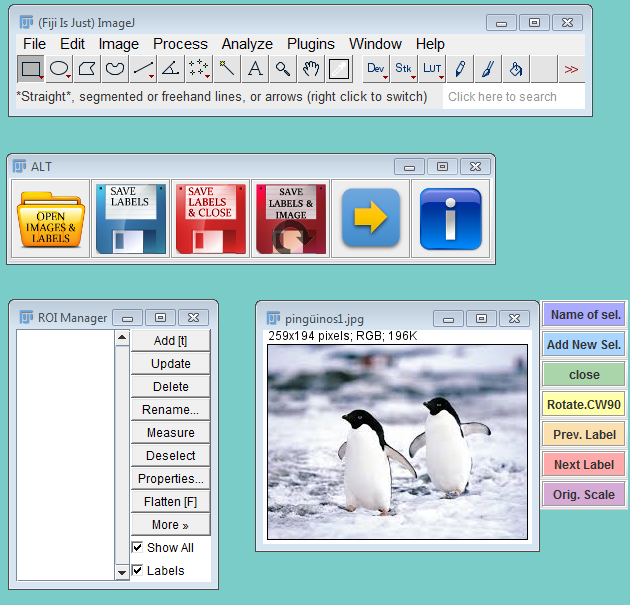
\includegraphics[width=0.7\linewidth]{img/etiquetado0}
		\caption{Estado de la aplicación antes del etiquetado}
		\label{fig:etiquetado0}
	\end{figure}
	
	\item \textbf{Etiquetado.} Para realizar el etiquetado dentro de una imagen que previamente hemos cargado tenemos que dibujar un rectángulo con el puntero sobre dicha imagen.
	Vamos a ponerle nombre a la etiqueta que hemos dibujado, para ello, una vez dibujado el rectángulo, pulsamos \textit{Add New Sel} en la columna de botones que hay a la derecha de la imagen. Ver imagen \ref{fig:etiquetapingu}.
	\begin{figure}
		\centering
		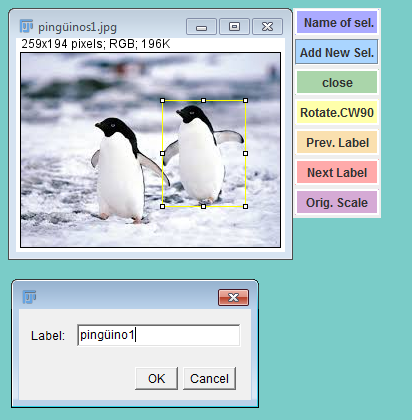
\includegraphics[width=0.7\linewidth]{img/etiquetapingu}
		\caption{Nombrar una etiqueta}
		\label{fig:etiquetapingu}
	\end{figure}
	
	En el caso de que después necesitásemos saber el nombre de la etiqueta que hemos puesto, manteniendo la etiqueta seleccionada, le damos a \textit{Name of sel} y nos dirá el nombre.
	\item \textbf{Guardar imágenes y etiquetas.} Una vez lo tenemos todo etiquetado dentro de la imagen tenemos que guardar la información generada por el etiquetado.
	Para llevar esto a cabo tenemos tres opciones: Guardar sólo las etiquetas y continuar etiquetando, guardar etiquetas y salir o guardar etiquetas e imágenes.
	Preferiblemente vamos a darle a la opción (en el menú ALT) de guardar etiquetas e imágenes y guardar todas las etiquetas en la misma carpeta de resultados para trabajar mejor con ellas.
	\item \textbf{Generar datos.}
	
\end{itemize}
\subsubsection{Recomendaciones}
He subido una máquina virtual a One Drive para que no sea necesario hacer ninguna instalación. Se puede acceder a la descarga desde \href{https://universidaddeburgos-my.sharepoint.com/:f:/g/personal/mmb0093_alu_ubu_es/EmokrIxFowNKvCanhqclkqkB90ruM7w-TPeXQS1MQQNmCQ?e=HMXXW4}{aquí}.